\documentclass[../dropout-vs-batch-normalization.tex]{subfiles}

\begin{document}

\subsection{Benchmark Datasets}

We carry out experiments and comparisons on two benchmark image classification datasets: MNIST~\cite{LeCun1999} and CIFAR-10~\cite{Krizhevsky2009}.

\medskip
\subsubsection{MNIST: Handwritten Digits}

MNIST (Modified National Institute of Standards and Technology)~\cite{LeCun1999} is a set of 60,000 training and 10,000 test images of handwritten digits from 0 to 9. All images are 28x28 pixels in grayscale, with the digits centered in the image.

It was created by combining a subset of two NIST digit sets, one containing digits from employees of the Census Bureau, and one containing digits from high-school students. These sets were chosen to provide a mix of samples that are considered easy to classify (the ones from the Census Bureau employees) and samples that are relatively harder to classify (the ones from the high-school students).

To make the validation process more meaningful the training and test sets were split by the original writers in a way that they do not overlap (digits from a given writer are either in the training set or the test set, but not in both) and the two types of writers are equally represented (half of the samples in the training and test set comes from the Census Bureau employees, the other half from the high-school students). This careful split results in a robust evaluation of a trained model (it will be presented with samples from writers it has not been trained on).

Figure~\ref{fig:MnistExamples} shows a sample of the MNIST dataset.

\begin{figure}[!htbp]
\centerline{\includegraphics[width=0.9\columnwidth]{figures/figures-other/MnistExamples.png}}
\caption{Sample handwritten digits of the MNIST (Modified National Institute of Standards and Technology) dataset. Each row represents a digit written in different styles.}
\label{fig:MnistExamples}
\end{figure}

\medskip
\subsubsection{CIFAR-10: Natural Images}

CIFAR-10 (Canadian Institute For Advanced Research) dataset~\cite{Krizhevsky2009} is a collection of natural images that are commonly used to train machine learning and computer vision algorithms. The dataset contains 50,000 training images and 10,000 test images. All images are 32x32 pixels in color (RGB channels). The dataset has 10 classes of images, representing airplanes, cars, birds, cats, deer, dogs, frogs, horses, ships, and trucks, as shown in Fig.~\ref{fig:CifarSample}. The training set has 5,000 images in each class, and the test set has 1,000 images in each class.

The set was created from images collected from the internet and manually labeled by humans. The creation process ensured that no duplicates or synthetically-created images are present in the set.

Figure~\ref{fig:CifarSample} shows a sample of the CIFAR-10 dataset.

\begin{figure}[!htbp]
\centerline{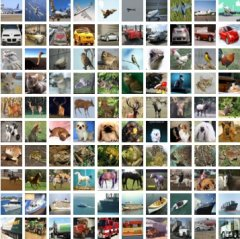
\includegraphics[width=0.9\columnwidth]{figures/figures-other/cifar10.png}}
\caption{CIFAR-10 (Canadian Institute For Advanced Research) sample images \cite{KrizhevskyCifar}. Each row represents a type of objects (airplanes, cars, birds, cats, deer, dogs, frogs, horses, ships, or trucks) under different background or visual appearance.}
\label{fig:CifarSample}
\end{figure}

\subsection{Deep Learning Algorithms}

We carry out comparisons using two types of deep learning architectures, multilayer perceptron networks (MLPs) and convolutional neural networks (CNNs) with different hyperparameter configurations. The architectures of the networks are detailed in Section~\ref{sec:results}.

\medskip
\subsubsection{MLP: Multilayer Perceptron Network}

Multilayer perceptron networks are networks composed of several fully connected layers. An example is shown in figure~\ref{fig:MlpStandardModel}.

The MNIST dataset was used to test the MLP networks and hyperparameters combinations. MNIST was chosen for this test because the original Dropout paper~\cite{Srivastava2014} also used MNIST in their MLP tests and formulated their guidelines for hyperparameters based on that. The Dropout paper recommends ranges of values for hyperparameters, including number of layers (2 to 4), number of units in the hidden layer (1024 to 4096 and a special case of 8192), learning rate (10x to 100x what would normally be used without Dropout), max-norm (3 to 4), among others.

We tested these combinations to document the effect they have on the network. The goal is to test combinations of the recommendations from that paper, verifying how they affect the training performance and the accuracy of the training model of an MLP network.

\medskip
\subsubsection{CNN: Convolutional Neural Network}

Convolutional neural networks are networks composed of several convolution and max-pooling layers. An example is shown in figure~\ref{fig:CnnStandardModel}.

CNN was used to test the CIFAR-10 dataset in the Dropout paper~\cite{Srivastava2014}. The Batch Normalization paper~\cite{Ioffe2015} used the ImageNet dataset for a similar test. For simplicity, given the hardware and time available for the tests performed here, CIFAR-10 (instead of ImageNet) was used for the Batch Normalization tests. Since the goal is to compare the relative performance of the strategies and hyperparameters, using CIFAR-10 should suffice in this application.

\subsection{Performance Metrics}

In order to comparatively study the model performance, the following performance measurements are collected in our experiments.

\medskip
\subsubsection{Training CPU time}

Training CPU time records the total CPUs and GPUs used to run all training epochs. Our goal is to measure how much system resources a network configuration uses during the training phase. 
 
This performance metric is used to understand how taxing the training phase is for a network configuration. Lower values are desirable to allow efficient use of expensive GPUs and to speed up the experimental phase, where different hyperparameter combinations have to be tried to find an optimal one.

In our experiments, we collected the training CPU time using the Python \verb|time| package, which measures the time to it took to execute Keras' \verb|model.fit(...)| function for the network configuration.

It is worth noting that for systems with more than one CPU or GPU this is not the same as clock (wall) time. Using a simplified example: if a network needs 20 seconds to be trained, in a system with two CPUs the training will complete in about 10 seconds. This item will report 20 seconds in this case. Measuring total CPU and GPU utilization gives a better view of the utilization of systems resources. Measuring only the clock time (10 seconds in this example) would not give an idea of how taxing the training phase really is on the system.

\medskip
\subsubsection{Test CPU time}

Test CPU time records the total amount of time used across all CPUs and GPUs to evaluate the trained network using the test set. Our goal is to capture the amount of system resources the trained network uses when it is evaluating samples. 

Test CPU time can help understand how efficient (or not) the trained network is on the end-users' systems. Lower variables are desirable here to be responsive to the end-user and, perhaps more importantly nowadays, to make efficient use of batteries in portable devices (e.g. phones).

Similar to the training CPU time, we collect the test CPU time using Python \verb|time| package, measuring the time to it took to execute Keras' \verb|model.evaluate(...)| function on the trained network. (similar to the training CPU time, this is not the same as clock (wall) time. See the note for that item for more details).

\medskip
\subsubsection{Number of parameters in the model}

Number of model parameters record the number of parameters the model has. Our goal is to evaluate and compare how much memory the model uses.

While deep learning normally emphasizes the model accuracy, the model size, in terms of number of parameters, provides a second metric to decide among models that have the same accuracy. The model with fewer parameters should be used because it will be faster to experiment with (run more training experiments), will use less memory on an end-user's device (and thus contribute to overall performance device by not forcing the operating system to eject other processes from memory) and use less battery (because it executes fewer calculations to predict the output.

In the experiments, we use Keras' \verb|model.count_params()| function, called on the model object after all layers have been created. Note that this number includes non-trainable parameters, such as auxiliary variables used in Batch Normalization. Therefore size at test time is an approximation (but it is close enough).

\medskip
\subsubsection{Training and validation loss and accuracy for each epoch}

This performance metric records the training loss and shows whether the network is improving as training progresses and how fast it is doing so. The validation loss checks if the network is overfitting or underfitting. Our goal is to measure how fast the network converges and if the network will perform well on unseen data.

Given two models that have the same accuracy, the one that achieves that accuracy faster (fewer epochs) saves system resources at training time (assuming a technique to decide that in real-time, such as early stopping, is being used) and allows faster experimentation cycles. Therefore, this measure allow us to have a measurement for training efficiency among the models tested.

In the experiments, we collect the results by setting the parameter \verb|validation_data| when executing Keras' \verb|model.fit(...)|. Keras returns a \verb|History| object when validation data is supplied. This object contains the training and validation loss and accuracy for each training epoch. Note that the code uses the test portion of the datasets for this purpose. Since the code is not making decisions based on that (\textit{e.g.} early stopping~\cite{Morgan1989} or annealing the learning rate), this is an acceptable practice. \cite{KerasTeam2016} has a similar discussion for this usage pattern in the Keras examples.

\subsection{Testing Environment}

All experiments reported in the paper were carried out on a Google Cloud virtual machine with the following specification

\medskip
\subsubsection{Machine Configuration}

\begin{itemize}
\item Machine type: n1-standard-4
\item Number of CPUs: 4
\item Memory: 15 GB
\item GPU: 1 x NVIDIA Tesla P100
\end{itemize}

The base image used for this virtual machine was \textit{Intel\textsuperscript{\textregistered} optimized Deep Learning image}, described by Google Cloud as \textit{A Debian based image with TensorFlow (With CUDA 10.0 and Intel\textsuperscript{\textregistered} MKL-DNN, Intel\textsuperscript{\textregistered} MKL) plus Intel\textsuperscript{\textregistered} optimized NumPy, SciPy, and scikit-learn.}

Using a GPU was essential to explore the combination of hyperparameters described in the following sections. Training was 30x faster in that environment, compared to a relatively high-performing machine without a GPU (Intel i7 2.9 GHz, 16 GB RAM).

\medskip
\subsubsection{Programming Tools}

The following programming tools were used to implement the empirical study framework and the experiment designs:

\begin{itemize}
\item Python 3.5.3
\item Keras 2.2.4
\item TensorFlow 1.12.0 (with GPU support enabled)
\end{itemize}

\end{document}
